\begin{pa} \label{PA:10.6} 
  Let's consider the function $f$ defined by 
  $$
  f(x,y) = 30 - x^2 - \frac 12 y^2,
  $$
  and suppose that $f$ measures the temperature, in degrees Celsius, at a given point in the plane, where $x$ and $y$ are measured in feet.  Assume that the positive $x$-axis points due east, while the positive $y$-axis points due north.  A contour plot of $f$ is shown in Figure \ref{F:10.6.preview.1}

  \begin{figure}[ht]
    \begin{center}
      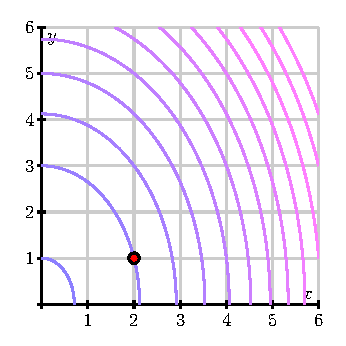
\includegraphics{figures/fig_10_6_preview_1.eps}
    \end{center}
    \caption{A contour plot of $f(x,y) = 30-x^2-\frac12 y^2$.}
    \label{F:10.6.preview.1}
  \end{figure}
  \ba
  	\item Suppose that a person is walking due east, and thus parallel to the $x$-axis.  At what instantaneous rate is the temperature changing at the moment she passes the point $(2,1)$?  What are the units on this rate of change?
	\item Next, determine the instantaneous rate of change of temperature at the point $(2,1)$ if the person is instead walking due north.  Again, include units on your result.
	\item Now, rather than walking due east or due north, let's suppose that the person is walking with velocity given by the vector $\vv = \langle 3, 4 \rangle$, where time is measured in seconds.  Note that the person's speed is thus $| \vv | = 5$ feet per second.
	
	Find parametric equations for the person's path; that is, parameterize the line through $(2,1)$ using the direction vector $\vv = \langle 3, 4 \rangle$.  Let $x(t)$ denote the $x$-coordinate of the line, and $y(t)$ its $y$-coordinate.
	
	\item With the parameterization in (c), we can now view the temperature $f$ as not only a function of $x$ and $y$, but also of time, $t$.  Hence, use the chain rule to determine the value of $\frac{df}{dt}\bigm|_{t=0}$.  What are the units on your answer?  What is the practical meaning of this result?
  \ea
  


\end{pa}

\begin{activitySolution} 
  \ba
  	\item The instantaneous rate of change in the temperature when a person is walking due east at the moment she passes the point $(2,1)$ is given by $f_x(2,1)$. Since $f_x(x,y) = -2x$, we have $f_x(2,1) = -4 \ \frac{^{\circ}C}{\text{foot}}$. 
  	
	\item The instantaneous rate of change in the temperature when a person is walking due north at the moment she passes the point $(2,1)$ is given by $f_y(2,1)$. Since $f_y(x,y) = -24 y$, we have $f_y(2,1) = -24 \ \frac{^{\circ}C}{\text{foot}}$. 
	
	\item Parametric equations for the line through $(2,1)$ in the direction of $\vv = \langle 3, 4 \rangle$ are
\[x(t) = 2 + 3t \ \text{ and } \ y(t)=1+4t.\]
	
	\item With the parameterization in (c), we have 
\[\frac{df}{dt} = \frac{\partial f}{\partial x} \frac{dx}{dt} + \frac{\partial f}{\partial y} \frac{dy}{dt} = (-2x)(3) - (24y)(4).\]
So
\[\frac{df}{dt}\biggm|_{t=0} = (-2)(2)(3) - (24)(1)(4) = -108 \ \frac{^{\circ}C}{\text{second}}.\]
So the temperature is decreasing by 108 degrees Celsius for every second she moves in the direction of $\vv$ from the point $(2,1)$. 
  \ea
\end{activitySolution}

 \afterpa 